% =====================================================================
%  Informe de avance del producto de software — Proyecto OLA
%  Formato IEEE (IEEEtran, modalidad conference) en español.
%  Compilar: pdflatex -> bibtex -> pdflatex -> pdflatex
%  (en Overleaf basta con subir la carpeta completa y compilar)
% =====================================================================
\documentclass[conference,a4paper]{IEEEtran}
\IEEEoverridecommandlockouts

\usepackage[T1]{fontenc}
\usepackage[utf8]{inputenc}
\usepackage{babel}
\babelprovide[import,main]{spanish}
\setlocalecaption{spanish}{table}{Tabla}
\setlocalecaption{spanish}{abstract}{Resumen}

\usepackage{cite}
\usepackage{amsmath,amssymb}
\usepackage{graphicx}
\usepackage{booktabs}
\usepackage{multirow}
\usepackage{array}
\usepackage{siunitx}
\sisetup{output-decimal-marker={.},group-separator={,},group-minimum-digits=4}
\usepackage[table]{xcolor}
\usepackage{tikz}
\usetikzlibrary{arrows.meta,positioning,fit,backgrounds}
\usepackage{algorithm}
\usepackage{algpseudocode}
\usepackage{url}
\usepackage[hidelinks]{hyperref}

\renewcommand{\IEEEkeywordsname}{Palabras clave}
\floatname{algorithm}{Algoritmo}
\algrenewcommand\algorithmicrequire{\textbf{Entrada:}}
\algrenewcommand\algorithmicensure{\textbf{Salida:}}
\newcolumntype{L}[1]{>{\raggedright\arraybackslash}p{#1}}
\definecolor{abisal}{HTML}{0A2530}
\definecolor{marea}{HTML}{1F6F80}
\definecolor{espuma}{HTML}{E3EEF0}

\begin{document}

\title{OLA: Observatorio Litoral de Anomalías Térmicas\\
\large Informe de avance de un sistema web de monitoreo y alerta de la temperatura superficial del mar desarrollado bajo un proceso de aseguramiento de la calidad}

\author{
\IEEEauthorblockN{Frederick Mares Graos, Jhordan Huamani Huamani, Jorge Ortiz Castañeda,\\ Miguel Angel Flores Leon y Piero Adrian Delgado Chipana}
\IEEEauthorblockA{Escuela Profesional de Ingeniería de Software, Facultad de Ingenierías y Arquitectura\\
Universidad La Salle, Arequipa, Perú\\
Curso de Calidad de Software (3.8.2.21) --- Docente: Maribel Molina Barriga}
}

\maketitle

% ---------------------------------------------------------------------
\begin{abstract}
El Instituto del Mar del Perú (IMARPE) publica como dato abierto la anomalía diaria de la temperatura superficial del mar (ATSM) de sus laboratorios costeros, pero en un formato que solo aprovechan los especialistas. Este informe presenta el avance de OLA, una aplicación web que clasifica el estado térmico de los 10 laboratorios costeros del litoral peruano en cálido, neutro o frío, lo muestra en un mapa interactivo, grafica y compara su histórico desde 1970, estima la tendencia de los próximos días con dos modelos simples y avisa por correo a los usuarios suscritos cuando una zona mantiene una anomalía sostenida. El proyecto se desarrolló con Scrum y con un proceso de calidad basado en IEEE~830, ISO/IEC~25010 y una estrategia de pruebas por capas. Al cierre de este avance, los ocho requisitos funcionales están implementados y verificados por 943 pruebas automatizadas, con una cobertura del 95\,\% en el backend y sin violaciones serias de accesibilidad WCAG~2.2~AA. Con el dataset completo (\num{125701} registros) la importación tarda \SI{11.8}{s} y el mapa se muestra en \SI{1.07}{s} con una red 4G, frente a límites de \SI{120}{s} y \SI{3}{s}. El análisis previo de los datos reales obligó a precisar cinco de los ocho requisitos, y las pruebas detectaron defectos que habrían pasado inadvertidos, entre ellos una verificación de tipos que no revisaba ningún archivo.
\end{abstract}

\begin{IEEEkeywords}
anomalía de la temperatura superficial del mar, calidad de software, ingeniería de requisitos, ISO/IEC 25010, pruebas automatizadas, sistemas de alerta temprana, accesibilidad web.
\end{IEEEkeywords}

\renewcommand{\abstractname}{Abstract}
\begin{abstract}
The Peruvian Sea Institute (IMARPE) publishes the daily sea surface temperature anomaly (SSTA) of its coastal laboratories as open data, in a format only specialists can use. This progress report presents OLA, a web application that classifies the thermal state of Peru's 10 coastal laboratories as warm, neutral or cold, displays it on an interactive map, charts and compares their history since 1970, estimates the short-term trend with two simple models, and emails subscribed users when a zone shows a sustained anomaly. The project followed Scrum and a quality process based on IEEE~830, ISO/IEC~25010 and a layered testing strategy. All eight functional requirements are implemented and verified by 943 automated tests, with 95\,\% backend coverage and no serious WCAG~2.2~AA violations.
\end{abstract}

\begin{IEEEkeywords}
sea surface temperature anomaly, software quality, requirements engineering, automated testing, early warning systems.
\end{IEEEkeywords}

% ---------------------------------------------------------------------
\section{Introducción}

El litoral peruano, bajo la influencia del sistema de la corriente de Humboldt, es muy sensible a las variaciones de la temperatura del mar. Un calentamiento o enfriamiento sostenido altera la disponibilidad de los recursos pesqueros y, con ella, la economía de miles de pescadores artesanales. El Niño Costero de 2017 afectó la salud y el bienestar de unos 1.9 millones de peruanos, causó 169 muertes y restó 1.5 puntos porcentuales al crecimiento del PIB de ese año; los modelos climáticos globales no lograron predecirlo ni con un mes de anticipación~\cite{yglesias2023}.

IMARPE mide a diario la temperatura del mar en sus laboratorios costeros y publica la anomalía en la Plataforma Nacional de Datos Abiertos~\cite{imarpe_dataset}. El dato es público, pero llega como un archivo de más de cien mil filas, sin clasificar y con retrasos y huecos que un lector no especialista no puede advertir. No existe tampoco un mecanismo que avise a quien sigue una zona concreta cuando la temperatura se aparta de lo normal de forma sostenida.

OLA (Observatorio Litoral de Anomalías térmicas) responde a esa brecha con una aplicación web móvil primero que traduce el dato a un lenguaje sencillo. El proyecto es además el trabajo práctico del curso de Calidad de Software, por lo que su objetivo secundario es demostrar un proceso de calidad aplicado a lo largo de todo el desarrollo. OLA es una herramienta complementaria: no reemplaza los boletines de IMARPE ni pronostica eventos El Niño, función que corresponde al ENFEN~\cite{enfen2024}.

Las contribuciones de este avance son: (i) un catálogo de requisitos trazable, refinado a partir del análisis del dataset real; (ii) un sistema funcional que implementa los ocho requisitos funcionales comprometidos; y (iii) evidencia cuantitativa de calidad (pruebas, cobertura, rendimiento y accesibilidad) vinculada a cada requisito.

El resto del informe se organiza así: la Sección~\ref{sec:marco} resume el marco teórico; la~\ref{sec:metodo}, la metodología; la~\ref{sec:req}, los requisitos; la~\ref{sec:diseno}, la arquitectura y los algoritmos; la~\ref{sec:avance}, el avance del producto; la~\ref{sec:eval}, la evaluación de calidad; y las Secciones~\ref{sec:disc} y~\ref{sec:concl}, la discusión y las conclusiones.

% ---------------------------------------------------------------------
\section{Marco teórico y trabajos relacionados}\label{sec:marco}

\subsection{Anomalía térmica y El Niño Costero}
La ATSM es la diferencia entre la temperatura medida y su valor climatológico para la misma fecha y lugar. En el Perú, el ENFEN define los eventos El Niño y La Niña costeros a partir del Índice Costero El Niño (ICEN), una media móvil de tres meses de la anomalía en la región Niño~1+2~\cite{reupo2024,enfen2024}. OLA no calcula el ICEN: trabaja con la anomalía diaria de cada laboratorio y adopta un umbral de $\pm$\SI{0.5}{\celsius} para separar el estado neutro de los estados cálido y frío, como criterio simple y configurable.

\subsection{Detección de eventos sostenidos}
La literatura sobre olas de calor marinas define un evento como un periodo en que la temperatura supera un umbral durante al menos cinco días, y admite huecos cortos dentro del mismo evento~\cite{capotondi2024}. OLA sigue la misma idea: un episodio de alerta exige una racha mínima de registros fuera del rango neutro (cinco por defecto) y tolera hasta dos días faltantes entre mediciones, porque el dataset de IMARPE tiene huecos frecuentes.

\subsection{Información para comunidades pesqueras}
En la pesca artesanal peruana, el celular es el medio de comunicación habitual: en la Cuarta Encuesta Estructural de la Pesquería Artesanal (ENEPA~IV, 2022--2023), solo el 29.9\,\% de las embarcaciones tenía radio a bordo, porque la mayoría usa el celular~\cite{enepa2025}. Además, durante El Niño Costero de 2017 las barreras de lenguaje y una difusión inadecuada impidieron que la población entendiera los pronósticos y las alertas, lo que dificultó la respuesta~\cite{yglesias2023}. Ambos hechos respaldan la decisión de diseñar OLA para el celular y de comunicar los estados con palabras de la costa en lugar de términos técnicos.

\subsection{Calidad de software}
La especificación de requisitos sigue IEEE~830 y las buenas prácticas de ISO/IEC/IEEE~29148, y documenta cada requisito en una ficha: una plantilla de formulario con sus atributos~\cite{ireb2024}. Los atributos no funcionales se organizan según el modelo de calidad de producto de ISO/IEC~25010~\cite{iso25010}. Las pruebas siguen la pirámide de pruebas~\cite{istqb2024}: muchas pruebas unitarias rápidas, menos de integración y pocas de extremo a extremo. La accesibilidad se mide contra WCAG~2.2~\cite{wcag22}, y la distinción de series para personas con daltonismo se valida con simulación de deficiencias de la visión del color~\cite{jamil2024}.

% ---------------------------------------------------------------------
\section{Metodología}\label{sec:metodo}

\subsection{Organización del trabajo}
El equipo de cinco integrantes trabajó con Scrum~\cite{scrum2025}, con un Product Owner, un Scrum Master que también actúa como responsable de QA y tres desarrolladores. El semestre se divide en siete sprints de dos semanas y dos hitos de control: el Hito~1 (catálogo de requisitos y avance del producto), al que corresponde este informe, y el Hito~2 (artículo final, prototipo y presentación).

\subsection{Ingeniería de requisitos}
El catálogo inicial definió ocho requisitos funcionales (RF-01 a RF-08) con un límite de ocho impuesto por el enunciado del curso. Antes de escribir código se analizó el archivo real de IMARPE. Ese análisis reveló cinco hechos que la especificación daba por sentados de otra manera (Tabla~\ref{tab:dataset}) y motivó seis versiones controladas del catálogo, cada una registrada con fecha, requisito afectado y motivo.

\begin{table}[!t]
\centering
\caption{Hallazgos del análisis del dataset y su efecto en los requisitos}
\label{tab:dataset}
\footnotesize
\begin{tabular}{@{}L{3.6cm}L{4.2cm}@{}}
\toprule
\textbf{Hallazgo} & \textbf{Consecuencia}\\
\midrule
\num{125701} filas de 1970 a 2026, no las $\sim$\num{3650} previstas & Carga por lotes y agrupado automático de series (RF-05, RF-08)\\
Archivo UTF-8 con marca de orden de bytes & El importador lee \texttt{utf-8-sig}\\
Matarani dejó de medir en 2016 & Estado «sin datos recientes» derivado de la fecha (RF-04)\\
Huecos de hasta \num{1127} días & Racha contada por registros; la línea del gráfico se corta (RF-01, RF-05)\\
El diccionario nombra un laboratorio inexistente en los datos & El catálogo de zonas se fija por migración y se rechazan laboratorios desconocidos (RF-08)\\
\bottomrule
\end{tabular}
\end{table}

\subsection{Estrategia de verificación}
Cada requisito se verifica en la capa donde su lógica vive. La lógica de dominio es pura: recibe listas y fechas explícitas, sin acceso a la base de datos ni al reloj, lo que hace sus pruebas rápidas y deterministas. Las pruebas de integración ejercitan los endpoints contra una base PostgreSQL separada. Como las bibliotecas de mapa y gráficos no pueden dibujarse en un DOM simulado, su comportamiento real se comprueba con pruebas de extremo a extremo en Chromium, en escritorio y en un celular emulado, que incluyen análisis de accesibilidad con axe y regresión visual. El correo se verifica con entrega real a un servidor de pruebas (Mailpit), no con un simulacro.

% ---------------------------------------------------------------------
\section{Requisitos del sistema}\label{sec:req}

La Tabla~\ref{tab:rf} resume los requisitos funcionales con su complejidad y su estado. El catálogo completo, con objetivos, actores, requisitos de información, 18 reglas de negocio, 14 casos de uso, 19 requisitos no funcionales y matrices de trazabilidad, se entrega como documento aparte.

\begin{table}[!t]
\centering
\caption{Requisitos funcionales y estado al Hito 1}
\label{tab:rf}
\footnotesize
\begin{tabular}{@{}lL{4.3cm}cc@{}}
\toprule
\textbf{ID} & \textbf{Requisito} & \textbf{Compl.} & \textbf{Estado}\\
\midrule
RF-01 & Detección de anomalía térmica sostenida & Alta & Verificado\\
RF-02 & Proyección de la tendencia a 3--7 días & Alta & Verificado\\
RF-03 & Notificación por correo y en la aplicación & Alta & Verificado\\
RF-04 & Mapa interactivo de las 10 zonas & Media & Verificado\\
RF-05 & Gráficos históricos por laboratorio & Media & Verificado\\
RF-06 & Comparación de 2 a 4 laboratorios & Media & Verificado\\
RF-07 & Registro, autenticación y suscripción & Baja & Verificado\\
RF-08 & Importación del CSV de ATSM & Baja & Verificado\\
\bottomrule
\end{tabular}
\end{table}

Los requisitos no funcionales principales son: carga del mapa en \SI{3}{s} o menos con 4G (rendimiento), importación de un año de histórico en menos de dos minutos, cumplimiento de WCAG~2.2~AA con ningún estado comunicado solo por color (capacidad de interacción), fecha del último dato siempre visible (fiabilidad), contraseñas con \emph{hash} bcrypt, tráfico HTTPS y rechazo a arrancar con secretos débiles (seguridad), y despliegue íntegro en contenedores (flexibilidad).

% ---------------------------------------------------------------------
\section{Arquitectura y diseño}\label{sec:diseno}

\subsection{Arquitectura}
OLA sigue una arquitectura cliente-servidor en capas (Fig.~\ref{fig:arq}). El frontend es una aplicación de una sola página en React, TypeScript y Vite, con Leaflet para el mapa y Recharts para los gráficos. El backend es una API REST en Python 3.13 con FastAPI, organizada en enrutadores, servicios, repositorios y un paquete de dominio puro. La persistencia usa PostgreSQL~17 con migraciones de Alembic. Todo se ejecuta en contenedores Docker y se despliega en un VPS Linux administrado con Dokploy, con Traefik como proxy HTTPS.

\begin{figure}[!t]
\centering
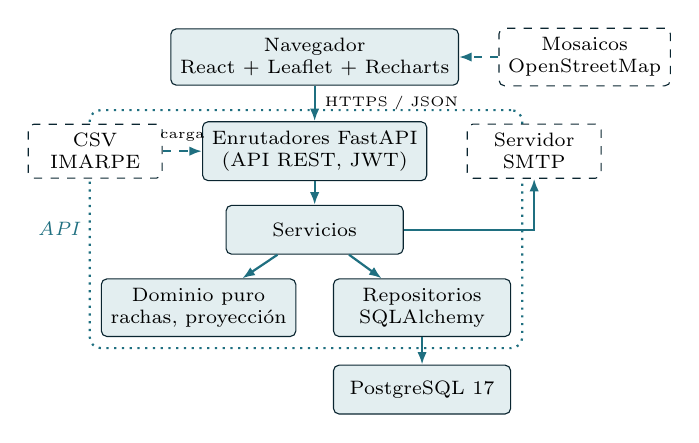
\begin{tikzpicture}[
  font=\scriptsize,
  caja/.style={draw=abisal, fill=espuma, rounded corners=2pt, minimum width=2.25cm, minimum height=0.62cm, align=center},
  ext/.style={draw=abisal, dashed, fill=white, rounded corners=2pt, minimum width=1.7cm, minimum height=0.62cm, align=center},
  flecha/.style={-{Latex[length=1.6mm]}, draw=marea, thick}]
\node[caja] (web) {Navegador\\React + Leaflet + Recharts};
\node[caja, below=0.45cm of web] (router) {Enrutadores FastAPI\\(API REST, JWT)};
\node[caja, below=0.3cm of router] (serv) {Servicios};
\node[caja, below left=0.3cm and -0.9cm of serv] (dom) {Dominio puro\\rachas, proyección};
\node[caja, below right=0.3cm and -0.9cm of serv] (repo) {Repositorios\\SQLAlchemy};
\node[caja, below=0.35cm of repo] (db) {PostgreSQL 17};
\node[ext, right=0.5cm of router] (smtp) {Servidor\\SMTP};
\node[ext, left=0.5cm of router] (csv) {CSV\\IMARPE};
\node[ext, right=0.5cm of web] (osm) {Mosaicos\\OpenStreetMap};
\begin{scope}[on background layer]
\node[draw=marea, dotted, thick, rounded corners, fit=(router)(serv)(dom)(repo), inner sep=4pt, label={[font=\scriptsize\itshape, text=marea]left:API}] {};
\end{scope}
\draw[flecha] (web) -- node[right, font=\tiny]{HTTPS / JSON} (router);
\draw[flecha] (router) -- (serv);
\draw[flecha] (serv) -- (dom);
\draw[flecha] (serv) -- (repo);
\draw[flecha] (repo) -- (db);
\draw[flecha] (serv.east) -| (smtp.south);
\draw[flecha, dashed] (csv) -- node[above, font=\tiny]{carga} (router);
\draw[flecha, dashed] (osm) -- (web);
\end{tikzpicture}
\caption{Arquitectura de OLA. El paquete de dominio no depende de la base de datos ni del reloj.}
\label{fig:arq}
\end{figure}

\subsection{Clasificación y fecha de referencia}
Sea $a$ la anomalía de una medición y $u$ el umbral (\SI{0.5}{\celsius} por defecto). La clasificación es
\begin{equation}
c(a)=\begin{cases}
\text{cálido} & \text{si } a>u,\\
\text{frío} & \text{si } a<-u,\\
\text{neutro} & \text{en otro caso,}
\end{cases}
\label{eq:clas}
\end{equation}
con límite exclusivo: una anomalía de exactamente $\pm u$ es neutra. Todos los cálculos usan como fecha de referencia $d_{\mathrm{ref}}$ la de la medición más reciente del sistema, no el reloj del servidor. IMARPE publica con retraso; con el reloj real, las diez zonas habrían aparecido «sin datos recientes» y el mapa entero en gris. Como efecto secundario, las pruebas son deterministas sin congelar el reloj.

El color de cada zona $z$ en el mapa sale del promedio de sus mediciones en una ventana de $w$ días (5 por defecto):
\begin{equation}
\bar{a}_z=\frac{1}{|M_z|}\sum_{m\in M_z} a_m,
\end{equation}
donde $M_z$ son las mediciones de $z$ con $d_{\mathrm{ref}}-w<d_m\le d_{\mathrm{ref}}$.
El promedio evita que un solo día atípico haga parpadear el estado. Una zona sin mediciones en los últimos 7 días no se clasifica.

\subsection{Detección de rachas}
El Algoritmo~\ref{alg:racha} recorre la serie de cada zona. Una racha crece mientras las mediciones conserven la misma clase no neutra y el número de días faltantes entre dos mediciones consecutivas no supere la tolerancia $g$. Un episodio se registra cuando la racha alcanza $k$ registros. La inserción de episodios usa una resolución de conflictos sobre (laboratorio, estado, fecha de inicio), de modo que reevaluar no duplica episodios ni cambia sus identificadores, condición de la que depende que los avisos no se reenvíen.

\begin{algorithm}[!t]
\caption{Detección de episodios sostenidos}
\label{alg:racha}
\small
\begin{algorithmic}[1]
\Require serie ordenada $(d_i,a_i)$, umbral $u$, racha mínima $k$, tolerancia $g$
\Ensure lista de episodios
\State $R\gets[\,]$; $E\gets[\,]$
\For{cada $(d_i,a_i)$}
  \State $s\gets c(a_i)$ \Comment{Ec.~\eqref{eq:clas}}
  \If{$s=$ neutro}
     \State \Call{Cerrar}{$R,E$}; $R\gets[\,]$
  \ElsIf{$R\neq[\,]$ \textbf{y} ($s\neq$ clase$(R)$ \textbf{o} $d_i-d_{\text{últ}}-1>g$)}
     \State \Call{Cerrar}{$R,E$}; $R\gets[(d_i,a_i)]$
  \Else
     \State agregar $(d_i,a_i)$ a $R$
  \EndIf
\EndFor
\State \Call{Cerrar}{$R,E$}
\Statex \textbf{procedimiento} \Call{Cerrar}{$R,E$}: si $|R|\ge k$, agregar a $E$ el episodio (inicio, fin, clase, $|R|$, pico)
\end{algorithmic}
\end{algorithm}

\subsection{Proyección a corto plazo}
Sobre las últimas $N=30$ mediciones de la zona se calculan dos modelos~\cite{hyndman2026}. La regresión lineal por mínimos cuadrados ajusta $\hat{a}(t)=\beta_0+\beta_1 t$ usando la fecha real $t$, de modo que los huecos pesen en la pendiente, y extrapola $h$ días (3 a 7, con 5 por defecto). La media móvil ponderada proyecta el nivel reciente:
\begin{equation}
\hat{a}_{\mathrm{MMP}}=\frac{\sum_{i=1}^{N} i\,a_i}{\sum_{i=1}^{N} i},
\end{equation}
donde $i=N$ es la medición más reciente (peso 30) e $i=1$ la más antigua (peso 1). La regresión sigue la \emph{dirección} de la serie y la media, su \emph{nivel}; cuando discrepan, esa diferencia se muestra al usuario como medida de incertidumbre. La confianza es alta si la cobertura de la ventana es de al menos 70\,\%, media si es de al menos 40\,\% y baja en otro caso o si el último dato supera la vigencia. El tramo estimado se marca con tres señales redundantes: trazo punteado, fondo sombreado y aviso en texto.

\subsection{Notificaciones}
La evaluación de alertas solo \emph{registra} los avisos pendientes (inicio y fin de cada episodio, uno por usuario y momento). El envío por SMTP es un paso separado, de forma que un servidor de correo lento o caído no bloquea la evaluación. Los envíos fallidos quedan marcados con su motivo y se reintentan en el siguiente intento.

% ---------------------------------------------------------------------
\section{Avance del producto}\label{sec:avance}

Al cierre de este avance, los ocho requisitos funcionales están implementados, integrados y desplegados. La Fig.~\ref{fig:inicio} muestra la pantalla principal: el resumen indica la fecha del último dato de IMARPE y su antigüedad, las zonas en alerta y el número de zonas por estado; el mapa representa cada zona con color, símbolo y nombre, y resalta con un anillo las que tienen una alerta vigente. La Fig.~\ref{fig:proy} muestra la proyección con las dos estimaciones, su diferencia y el indicador de confianza.

\begin{figure}[!t]
\centering
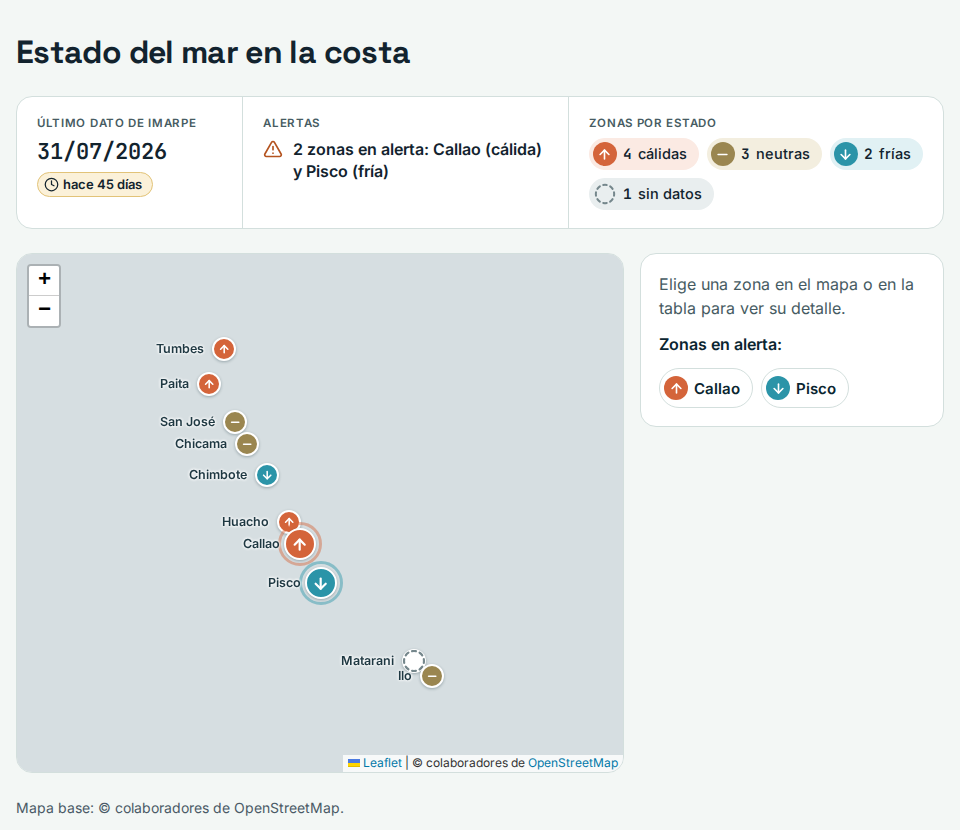
\includegraphics[width=\columnwidth]{figs/inicio-top.png}
\caption{Pantalla de inicio en escritorio con datos de prueba: resumen del estado, mapa de las 10 zonas y accesos a las zonas en alerta (RF-04).}
\label{fig:inicio}
\end{figure}

\begin{figure}[!t]
\centering
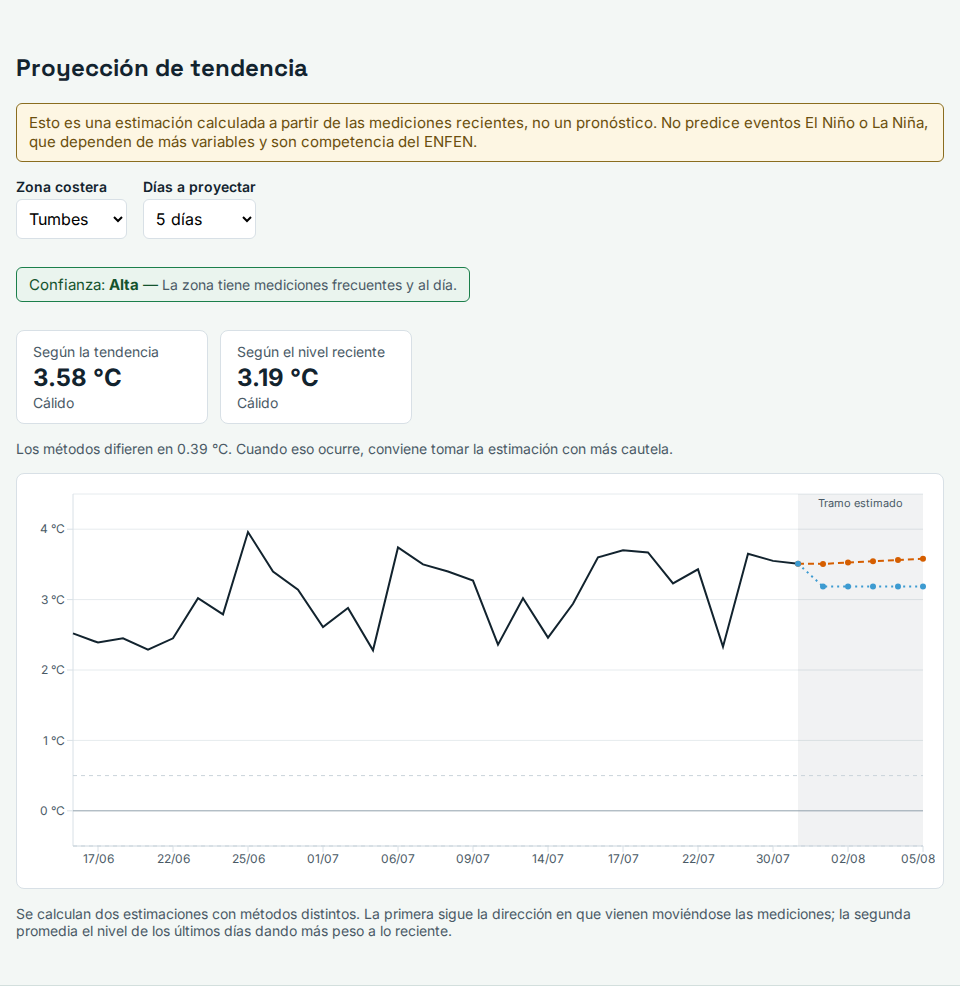
\includegraphics[width=0.92\columnwidth]{figs/proyeccion-chromium-linux.png}
\caption{Proyección de tendencia (RF-02): estimación por regresión y por media ponderada, confianza y tramo estimado sombreado.}
\label{fig:proy}
\end{figure}

La interfaz se rediseñó con un enfoque móvil primero: barra de navegación inferior en el celular, detalle de la zona en una hoja inferior modal, textos en lenguaje de la costa («sobre lo normal» en lugar de «anomalía positiva») y carga diferida de cada pantalla, que redujo la portada de 272 a \SI{170}{kB} comprimidos. El sistema completo se despliega con un único archivo de Docker Compose; las migraciones se ejecutan al arrancar bajo un bloqueo de PostgreSQL para que varias réplicas no migren en paralelo.

Con el dataset real, la evaluación detecta \num{4164} episodios desde 1970 en unos \SI{3}{s}, de los cuales 8 seguían vigentes a la fecha del último dato.

% ---------------------------------------------------------------------
\section{Evaluación de la calidad}\label{sec:eval}

\subsection{Pruebas y cobertura}
La Tabla~\ref{tab:pruebas} resume las suites. Las 943 pruebas se ejecutan en contenedores; el backend alcanza una cobertura del 95\,\% de las sentencias y pasa las herramientas ruff y mypy en modo estricto sin observaciones. El único módulo sin cobertura automática es el de arranque de producción, que se verificó levantando el \emph{stack} desde una base vacía.

\begin{table}[!t]
\centering
\caption{Suites de pruebas automatizadas}
\label{tab:pruebas}
\footnotesize
\begin{tabular}{@{}L{2.55cm}rL{3.75cm}@{}}
\toprule
\textbf{Suite} & \textbf{Pruebas} & \textbf{Alcance}\\
\midrule
Backend, unitarias & 212 & Dominio puro, sin base de datos\\
Backend, integración & 230 & Endpoints, persistencia, permisos\\
Frontend (Vitest) & 332 & Componentes y páginas, con axe\\
Extremo a extremo & 167 & Playwright en escritorio y celular, axe, regresión visual\\
Rendimiento & 2 & Playwright, build de producción con 4G\\
\midrule
\textbf{Total} & \textbf{943} & \\
\bottomrule
\end{tabular}
\end{table}

\subsection{Rendimiento y accesibilidad}
La Tabla~\ref{tab:rnf} compara las métricas medidas con los límites de la especificación. El tiempo del mapa se midió con la build de producción en un celular emulado con 4G (\SI{9}{Mbps}, \SI{40}{ms}) y la CPU ralentizada al doble, como mediana de tres cargas en frío. El análisis de accesibilidad con axe es bloqueante en todas las pantallas; la única excepción documentada es el tamaño de los marcadores del mapa (WCAG~2.5.8), cubierta por la misma selección disponible en tarjetas y tabla. La paleta de las series comparadas mantiene, con cuatro series simultáneas, una diferencia de color $\Delta E\ge 9.0$ en deuteranopía y un contraste de al menos 3:1 contra el fondo.

\begin{table}[!t]
\centering
\caption{Requisitos no funcionales medidos}
\label{tab:rnf}
\footnotesize
\begin{tabular}{@{}L{3.2cm}cc@{}}
\toprule
\textbf{Métrica} & \textbf{Límite} & \textbf{Medido}\\
\midrule
Mapa con 10 zonas (4G) & $\le$ \SI{3}{s} & \SI{1.07}{s}\\
Importación del dataset & $\le$ \SI{120}{s}/año & \SI{11.8}{s} (56 años)\\
Puntos por serie (56 años) & --- & $<$ \num{1000}\\
Portada comprimida & --- & \SI{170}{kB}\\
Violaciones serias de axe & 0 & 0\\
Cobertura del backend & --- & 95\,\%\\
\bottomrule
\end{tabular}
\end{table}

\subsection{Defectos detectados por el proceso}
Las pruebas encontraron defectos que habrían llegado a producción. Los más significativos fueron: un decimal escrito con coma que se cargaba en silencio con un valor erróneo; una fecha repetida que abortaba toda la importación; peticiones tardías que sobrescribían el resultado vigente al cambiar de zona; sesiones rechazadas de forma intermitente porque el reloj de la máquina virtual retrocedía, resuelto con una tolerancia de \SI{30}{s}; y dos procesos que chocaban al crear la cuenta de administrador. Dos defectos del propio proceso de pruebas resultaron los más instructivos: la verificación de tipos del frontend apuntaba a un archivo de configuración que no incluía archivos y pasaba sin revisar nada, y una tolerancia visual relativa del 0.5\,\% dejaba pasar cambios reales de texto.

% ---------------------------------------------------------------------
\section{Discusión}\label{sec:disc}

El proyecto se implementó antes de cerrar el catálogo de requisitos, que se formalizó y amplió después a partir del código, las pruebas y el registro de decisiones. Esta ingeniería inversa de requisitos tiene un riesgo claro: documentar lo construido en lugar de lo necesario. Para mitigarlo, cada requisito se contrastó con la problemática original, cada cambio de alcance quedó registrado con su motivo y cada criterio de aceptación se vinculó a pruebas que fallan si el comportamiento cambia.

La lección más útil fue leer los datos reales antes de diseñar. Cinco de los ocho requisitos cambiaron por hechos del dataset, y la mayoría de esos cambios hacen el sistema más honesto: marcar zonas sin datos recientes, cortar la línea en los huecos o bajar la confianza de una proyección con datos antiguos evita que el sistema aparente una certeza que no tiene. La segunda lección es que una prueba verde solo vale si verifica lo que se cree: dos de los defectos encontrados hacían que las pruebas pasaran sin comprobar nada.

Entre las limitaciones actuales están: la capacidad de 50 usuarios concurrentes no se ha verificado con una prueba de carga; no hay integración continua y las pruebas se ejecutan en local; la importación es solo manual; los modelos de proyección son deliberadamente simples y no constituyen un pronóstico; y cuatro pantallas conservan el estilo anterior al rediseño.

% ---------------------------------------------------------------------
\section{Conclusiones y trabajo futuro}\label{sec:concl}

OLA transforma un dataset público de difícil lectura en información útil para la pesca artesanal: el estado térmico de cada zona, su historia, una estimación de los próximos días y avisos cuando una anomalía se sostiene. Al Hito~1, los ocho requisitos funcionales están implementados y trazados a 943 pruebas automatizadas, y los requisitos de rendimiento y accesibilidad se cumplen con holgura.

Para el Hito~2 se prevé ejecutar una prueba de carga que verifique la capacidad concurrente, incorporar integración continua, extender el rediseño a las pantallas restantes y validar la comprensión de la interfaz con usuarios reales del perfil de pescador artesanal.

% ---------------------------------------------------------------------
\section*{Agradecimientos}
Al Instituto del Mar del Perú y al Ministerio de la Producción, por publicar el dataset de ATSM como dato abierto, y a los colaboradores de OpenStreetMap, por el mapa base.

\bibliographystyle{IEEEtran}
\bibliography{referencias}

\end{document}
